\chapter{Objectives and Contributions}
\label{chapter:objectives}

This chapter presents the main objectives of this thesis and identifies the contributions to the state of the art. We enumerate the assumptions considered in this work, describe the main hypotheses and draw the limit of the scope of the thesis presenting the restrictions. \cref{fig:chp3_summary} provides an overview of the objectives and contributions presented in this thesis, along with their relations with identified hypotheses, assumptions and restrictions. 

\section{Objectives}
\label{sec:chp3-objectives}

%% PREVIOUS
% improve the mapping languages regarding expressiveness, usage and adoption to comply with the current evolving needs in knowledge graph construction

%% CURRENT LONG VERSION
%To advance the state of the art of declarative KGC technologies regarding support in language expressiveness, mapping writing and their role in KG evolution.

The general objective of this thesis is to \textit{improve the understanding (features and limitations) and operational management of declarative KG construction languages}. In order to achieve this goal, the following sub-objectives are defined:

\begin{enumerate}
    %\item[\textbf{O1.}] To analyse, understand and gather the capabilities of the mapping languages for KG construction from heterogeneous data sources.
    \item[\textbf{O1}] To analyze the needs for declarative knowledge graph construction from heterogeneous data sources, in order to facilitate the support of advances in existing mapping languages to address the most relevant ones. 
    \item[\textbf{O2}] To help knowledge engineers and domain experts build declarative mappings in a user-friendly manner.
    \item[\textbf{O3}] To assess declarative knowledge graph construction technologies in terms of their benefits for supporting the creation and evolution of knowledge graphs. 
\end{enumerate}

In order to achieve the first objective, the following open research problem must be solved:
\begin{itemize}
    \item Ever since the first mapping languages began to be developed, many more have been proposed and released over the years. These languages address different needs and propose diverse features, but they share some characteristics, as in the end they all serve the same purpose of constructing KGs. In order to keep improving the KG construction process from heterogeneous sources, we need to identify which are the needs and the current challenges in the mapping languages. Thus we can facilitate the selection of languages according to their capabilities for addressing different needs. However, there is a lack of a fine-grained analysis of the competences and expressiveness of these mapping languages. %, as well as a formalization of their derived requirements. 
\end{itemize}

From a technological perspective, the following problem must be solved:
\begin{itemize}
    \item The needs for KG construction are not static, as they evolve with the use cases and evolution of surrounding technology. For instance, this is the case of the currently under development new specification of RDF 1.2~\parencite{hartig2023rdf}, that includes RDF-star triples. Mapping languages so far cannot produce RDF-star graphs without a dedicated extension, thus new technological support is needed to assist the creation of KGs with the evolving needs, and more specifically, to build RDF-star graphs. 
\end{itemize}

In order to achieve the second objective, the following research problem must be solved:
\begin{itemize}
    \item Most mapping languages are formalized as ontologies. In these cases, mappings are required to be written using an RDF serialization. Other common languages extend SPARQL to write transformation rules. This implies a double obstacle for new users, to learn the language and the language's syntax (i.e. Turtle or SPARQL) in case they are not familiar with them. There is a lack of methods that facilitate the writing process for both expert practitioners and new users to speed-up the process and become less error-prone.
    
    % while being up-to-date to the current needs in KG construction.
\end{itemize}

From a technological perspective, the following problem must be solved:
\begin{itemize}

    \item User-friendly approaches usually involve developing new syntaxes that cannot always be directly process by with KGC systems. In addition, different KGC systems are usually compliant with only one language. There is currently little interoperability among the existing languages, which limits the possibilities for users to use a wider variety of systems with different capabilities. Hence, new technological support is needed to allow translations among current mapping languages and reduce the barrier adoption enhancing the communication between user-friendly syntaxes and existing KGC implementations.   

\end{itemize}

Finally, for achieving the third objective, the following open research problem must be solved:

\begin{itemize}
    \item Knowledge graphs undergo a complex process from creation to consumption that comprise their life cycle. Declarative mapping rules and their supporting technologies are a key in the construction step, but can also play a beneficial role in other steps, such as data pre-processing and metadata annotation for transparency. However, there is a lack of research on their support in other tasks involved in the KG life cycle.
    %\textcolor{red}{Knowledge graphs are modeled according to schemes that are subject to changes over time. These modifications can be triggered by different factors, such as new requirements or error fixing, that can help improve the quality of the KG and the performance of downstream tasks that consume it. Graph re-construction can be achieved in different manners, but it is not known which approach perform best this task in different situations.} Thus, there is a lack of research on how mapping languages and compliant technology can assist this task to improve KG evolution. 
\end{itemize}

\section{Contributions}
\label{sec:chp3-contributions}

In this section, we describe the solutions corresponding to the objectives and open research problems described in \cref{sec:chp3-objectives}. We present as follows the contributions that support the advance of the current state of the art regarding the first objective (understand and gather the needs for KG construction): 

\begin{enumerate}
    \item[\textbf{C1}] Design of a \textbf{comparison framework analysing the state-of-the-art mapping languages} proposed to generate knowledge graphs from heterogeneous data sources. We extract the characteristics of these languages and compare them over a set of detailed features that show their expressiveness. 
    
    \item[\textbf{C2}] \textbf{Identification, definition and implementation of requirements for knowledge graph construction} from heterogeneous data sources. Based on the analysis performed on the comparison framework, we are able to extract what are the needs for building knowledge graphs, which are possible to achieve with the current languages and which need to be addressed yet. We implement these requirements in a formal language. 
    
    \item[\textbf{C3}] \textbf{Development of new features for the RML mapping language} to address the limitations of the language according to the new needs in knowledge graph construction. We focus on the development of the extension to create RDF-star graphs. 
\end{enumerate}

Regarding the second objective (to help knowledge engineers and domain experts to build mappings), we present new advances with the following contributions:

\begin{enumerate}
    \item[\textbf{C4}] \textbf{Design of a user-friendly approach for writing mapping rules based on spreadsheets}. We propose this approach as a way of writing mappings by only specifying the essential information, reducing learning curve of the language constructs and the syntax's peculiarities. We also develop an implementation of this approach to translate the mapping rules in spreadsheets into different mapping languages. 
    \item[\textbf{C5}] \textbf{Update of the YARRRML syntax for RML with new features}. We include in a new version of this syntax the features incorporated in the evolution of the RML mapping language, to keep this language accessible for a broader community of users that already use YARRRML. We also provide an implementation to translate between the updated YARRRML version into other mapping languages to facilitate its adoption.
\end{enumerate}

Finally, with regard to the third objective (to assess the role of mapping technologies in KG evolution), this work presents the following contribution:

\begin{enumerate}
    \item[\textbf{C6}]\textbf{Analysis of the scenarios in which declarative KG construction technologies play a valuable role in the refactoring of knowledge graphs}. We conduct an evaluation to study how mapping-based processes be beneficial when the schema used in a knowledge graph changes with respect to other established methods.  %can not only be useful for KG construction, but also for facilitating the evolution of knowledge graphs that need a change in their schema. 
\end{enumerate}


\section{Assumptions}
\label{sec:chp3-assumptions}
Our work is based on the set of assumptions listed below. These assumptions provide a background to facilitate the comprehension of the decisions taken during the development of this work. 


\begin{enumerate}
    \item[\textbf{A1}] Mapping languages are declarative.
    \item[\textbf{A2}] Mapping languages provide human readable documentation available online.
    \item[\textbf{A3}] The schema of knowledge graphs (ontology) used for creating mapping documents is available and implemented in OWL or RDF(S). 
    \item[\textbf{A4}] Mapping rules can be translated into different languages with information preservation. 
    \item[\textbf{A5}] The refactoring of the schema used in a KG does not involve changes in the data.
    %\item[\textbf{moar?}] KGs refer to RDF graphs?
\end{enumerate}


\section{Hypotheses}
\label{sec:chp3-hypotheses}

After the identification of the assumptions, we can describe the research hypotheses  of this thesis. They cover the general characteristics of the contributions:

\begin{enumerate}
    \item[\textbf{H1}] Current mapping languages lack some expressiveness to construct knowledge graphs from heterogeneous data sources for all use cases.
    \item[\textbf{H2}] It is possible to update  current mapping languages with new features that address the current needs in construction of knowledge graphs.
    \item[\textbf{H3}] Writing mapping rules in spreadsheet environments improves the user experience for practitioners of different backgrounds for writing mappings, whilst reducing errors. 
    \item[\textbf{H4}] Declarative KG construction technologies brings benefits in the refactoring of knowledge graphs within their life cycle.
\end{enumerate}


\section{Restrictions}
\label{sec:chp3-restrictions}

Finally, there is a set of restrictions that describe the limitations and define the future work objectives:

\begin{enumerate}
    \item[\textbf{R1}] Requirements for KG construction are considered up to January 2023, since it is an issue that is evolving during the time of writing this thesis.
    \item[\textbf{R2}] The reference for the RML specification in the mapping languages analysis is the release on 2014~\parencite{Dimou2014rml}.
    \item[\textbf{R3}] Features specific of non RDF-based mapping languages are not ensured to be modelled in an ontology (e.g. SPARQL recursive clauses and FILTER).
    \item[\textbf{R4}] The implementations proposed in contributions C4 and C5 are not fully compliant with all modules of the RML release on 2023~\parencite{iglesias2023rml}. 
    \item[\textbf{R5}] The evaluation of the value of mappings in KG refactoring considers only changes in the schema used in the KG, not in the data.
    \item[\textbf{R6}] The changes considered for KG refactoring are schema changes for switching among metadata representation approaches for RDF graphs.
    %\item[\textbf{moar?}] algo de la selección de lenguajes? algo para mapeathor y yarrrml? The spreadsheet template consider the features of RML v2014 and the current RML-FNML spec. The YARRRML updates include all RMLv2 modules except for the RML-CC module.
\end{enumerate}


\begin{sidewaysfigure}[t!]
    \centering
    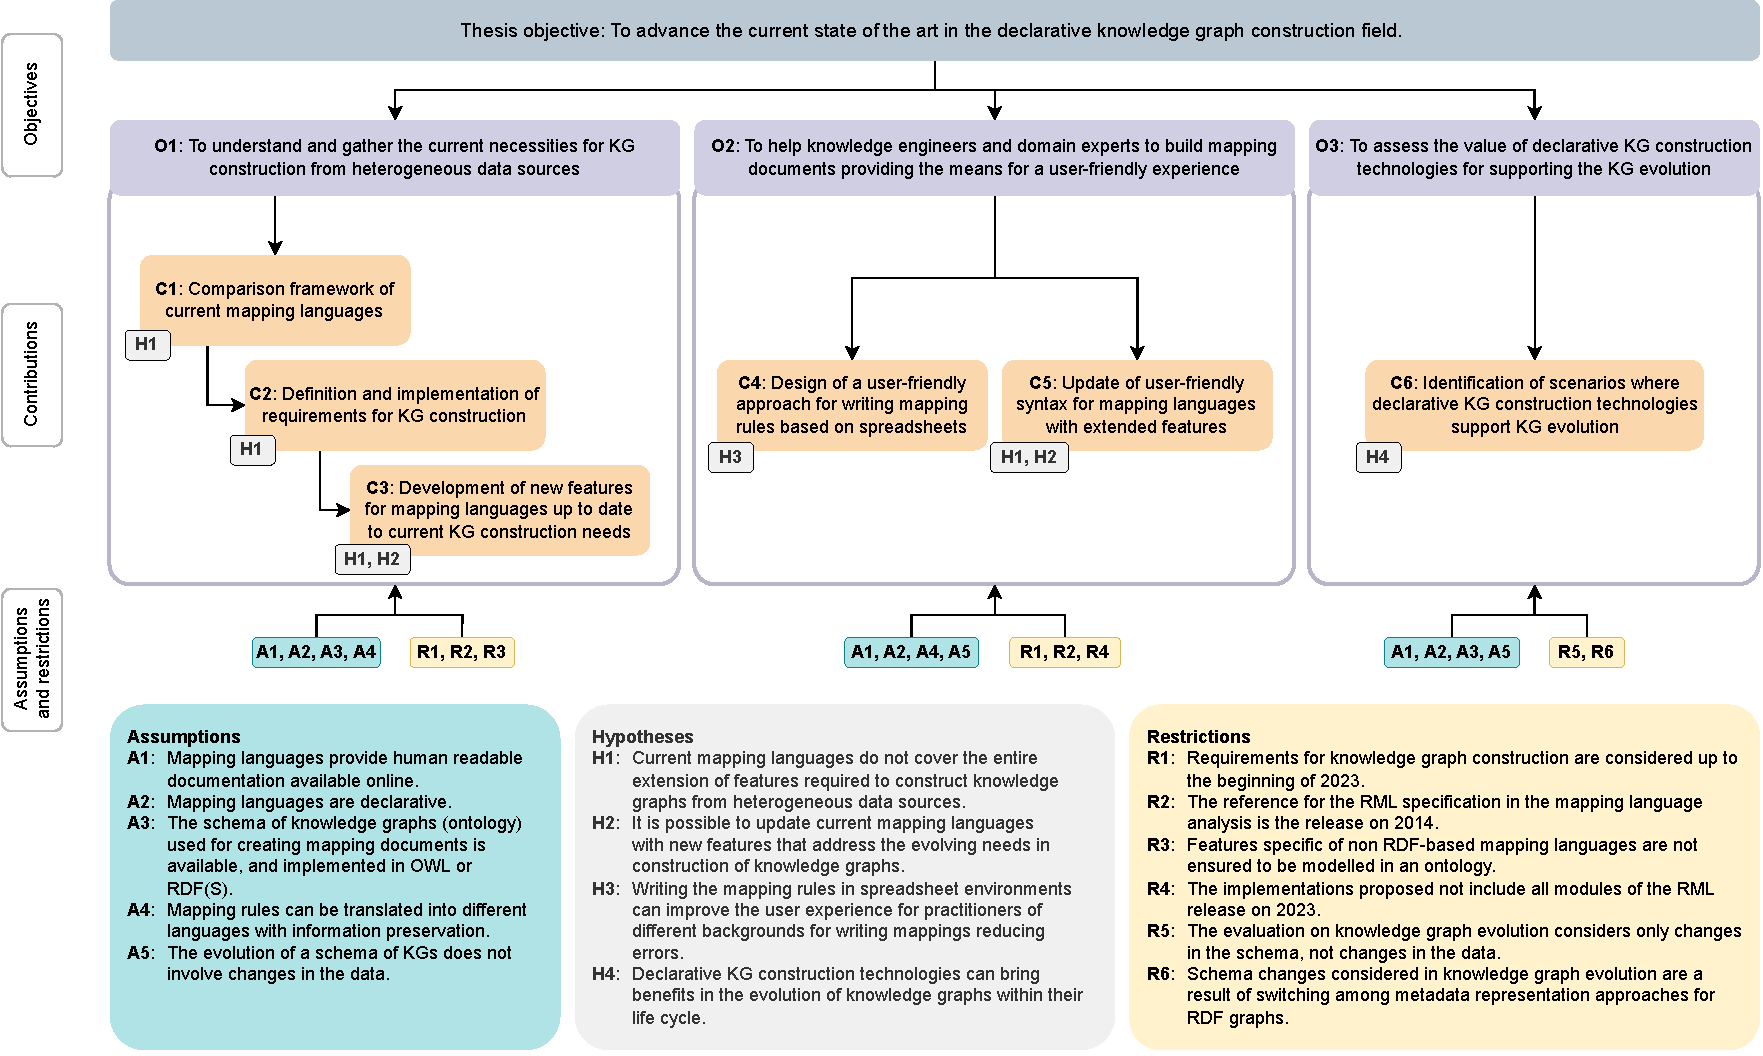
\includegraphics[width=1\linewidth]{figures/chp3_summary.pdf}
    \caption[Relations between objectives, contributions, hypotheses, assumptions and restrictions of this thesis]{Overview of objectives, contributions, hypotheses, assumptions and restrictions, and their relations.}
    \label{fig:chp3_summary}
\end{sidewaysfigure}

%\section{Research Methodology?}

